\chapter{Numerical Methods for Open Quantum Systems}
\label{chapter3}
\epigraph{Hilbert space is a big place.}{\textit{Carlton Caves}}
As we have seen in chapter~\ref{Chapter1}, the study of an open quantum system requires the knowledge of its density matrix, solution of the Lindblad master equation~\cite{presk:quant_info}:
\begin{equation*}
    \dot{\rho} = \mathcal{L}[\rho],
\end{equation*}
where
\begin{equation}
\label{eqn:lindblad_eqn}
    \mathcal{L}[\rho] \equiv -i[H, \rho] - \sum_{a=1}^{N^2-1}\gamma_a\Bigl(\frac{1}{2}L_a^{\dagger}L_a\rho + \frac{1}{2}\rho L_a^{\dagger}L_a - L_a\rho L_a^{\dagger}\Bigl),
\end{equation}
$N$ being the dimension of the Hilbert space.

In such a system the number of variables scales as the square of the dimension of the Hilbert space; for example, in a spin-$\frac{1}{2}$ system made up by $n$ elements, the size of the Hilbert space $\mathcal{H}$ is $2^n$ while the \emph{liouvillian dimension} equals to $2^{2n} \times 2^{2n}$. Clearly, a direct numerical integration of the equation~\ref{eqn:lindblad_eqn} can be made only for systems with a very limited number of elements. One only needs to note the fact that for a brute-force integration of the equation~\ref{eqn:lindblad_eqn} for a system consisting of $8$ sites, about $34$ GB of memory would be necessary\footnote{This calculation considers the fact that the liouvillian contains, in general, complex numbers, each of them valued with a single precision (32 bit).}.

Nevertheless, some techniques for exact diagonalization of the Liouvillian superoperator~\ref{eqn:lindblad_eqn} have been developed. Let us mention, for example, the one devised by Prosen~\cite{Prosen_2008}, for studying a system characterized by a quadratic Hamiltonian and linear Lindblad operators, which prescribes to diagonalize the Liouville super-operator in terms of $2n$ normal master modes, i.e. anticommuting super-operators which act on the Fock space of density operators. This can be understood as a complex version of the Bogoliubov transformation.

%The numerical methods employed in open quantum system problems can be classified in those that have a wave-function approach (quantum trajectories method, mean field method) and those that decompose the system into blocks (corner-space renormalization method, matrix product density operators method).

However, as seen previously, a direct integration of the master equation for an open many-body system becomes unfeasible even for relatively small sizes, so conceiving more clever numerical strategies seems to be necessary.

One of them is based on the \emph{mean field} approach; the essential idea is to consider the mean value of the Hamiltonian and, as suggested by Gutzwiller, to factorize the density matrix, defining a mean field density matrix $\rho_{MF} = \prod_j\rho_j$, where $\rho_j$ is the single site density matrix. In this way, all correlations and interactions between sites are neglected, so we can say it is a crude approximation for an interacting many-body system. In order to (partially) overcome this problem, the \emph{cluster mean field} method was developed: in this method a set of contiguous sites are isolated from the rest of the system. As explained in~\cite{jin_biella_ross}, this method suggests to write the Hamiltonian as $H_{CMF} = H_\mathcal{C} + H_{\mathcal{B(C)}}$, where the first term describes the exact interactions inside the cluster $\mathcal{C}$ while the second term represents the mean-field interactions between the cluster and the sites on its boundary $\mathcal{B(C)}$. The global density matrix will be $\rho_{CMF} = \bigotimes \rho_\mathcal{C}$, where the $\rho_\mathcal{C}$ is the density matrix of the $\mathcal{C}$-th cluster. One should note that, when the cluster is made up by a single site, the method becomes the above-mentioned standard one. 

Other important numerical methods are the ones essentially based on the \emph{linked cluster expansions}~\cite{oitmaa}, in which the quantities of interest are expressed as sums of contributions from a sequence of clusters of sites; in particular, only connected clusters contribute. In~\cite{PhysRevX.6.021037} an application of this idea to the Liouvillian is presented.

In this section, we will examine some of the numerical techniques used for studying open quantum systems with very different approaches.

Two of the three numerical methods analyzed in this chapter are essentially based on the Wilson's \emph{renormalization group} approach~\cite{RevModPhys.47.773} combined with the fundamental contribution of the White's \emph{density matrix renormalization group} (DMRG) method~\cite{s_white:dmrg} and are the \emph{corner-space renormalization} and the \emph{matrix product density operators} methods. They both use the idea of a system decomposition into blocks; even if the basic idea is the same, the developed approaches are actually different.

The first numerical method analyzed in the section~\ref{chapt3_qtm} is the \emph{quantum trajectories} method, based on the evolution of a Monte Carlo wave function.

%%%%%%%%%%%%%%%%%%%%%%%%%%%%%%%%%%%%%%%%%%%%%%%%%%%%%%%%%%%%%%%%%%%
%%%%%%%%%%%%%%%%%%%%%%%%%%%%%%%%%%%%%%%%%%%%%%%%%%%%%%%%%%%%%%%%%%%
%%%%%%%%%%%%%%%%%%%%%%%%%%%%%%%%%%%%%%%%%%%%%%%%%%%%%%%%%%%%%%%%%%%
\section{The Quantum Trajectories (QT) Method}
\label{chapt3_qtm}
The \emph{quantum trajectories method} is an estabilished numerical method, in which pure states are the subjects of the study, instead of density matrices. This means that, if the Hilbert space has dimension $N$, the number of involved parameters ($\sim N$) is much smaller than the one required in calculations with density matrices ($\sim N^2$). This method was originally proposed in 1992 by Dalibard, Castin and Mølmer in~\cite{PhysRevLett.68.580}, then generalized in~\cite{Molmer:93}, as a stochastic unraveling of the master equation, namely a stochastic evolution for the wave function of a system coupled to a reservoir. It has been proved~\cite{PhysRevLett.68.580, Molmer:93} that this \emph{Monte Carlo wave-function} approach is equivalent to the master equation treatment.

The idea of this method can be summarised in the following way.

First of all, given the~\ref{eqn:lindblad_eqn}, let us note that the first three terms of this equation can be regarded as the evolution performed by an effective non-Hermitian Hamiltonian, that is~\cite{PhysRevA.69.062317}:
\begin{equation}
    H_{\text{eff}} = H_s + \text{i}K,
\end{equation}
with
\begin{equation}
    K = -\frac{1}{2}\sum_\mu L_{\mu}^{\dagger}L_{\mu}.
\end{equation}
Indeed, we see that:
\begin{equation*}
    -\text{i}[H_\text{eff}, \rho] = -\text{i}[H_s, \rho] - \frac{1}{2}\sum_\mu \{L_{\mu}^{\dagger}L_{\mu}, \rho\}.
\end{equation*}

The summation term in the~\ref{eqn:lindblad_eqn}, is the one responsible for the so-called \emph{quantum jumps}; for this reason, the representation under which we have written the~\ref{eqn:lindblad_eqn} is called \emph{quantum jump picture}~\cite{PhysRevA.69.062317}. 

At an initial time $t_0$, the density matrix of the system is in a pure state
\[
\rho(t_0) = \ket{\phi(t_0)}\bra{\phi(t_0)};
\]
after a time $dt$, it evolves to the following statistical mixture:
\begin{equation}
    \rho(t_0 + dt) = \Bigl(1-\sum_\mu dp_\mu \Bigl)\ket{\phi_0}\bra{\phi_0} + \sum_\mu dp_\mu \ket{\phi_\mu}\bra{\phi_\mu},
\end{equation}
where
\begin{equation}
    dp_\mu = \bra{\phi(t_0)}L_{\mu}^{\dagger}L_{\mu}\ket{\phi(t_0)}dt
\end{equation}
is the probability that a jump occurs; in this case, the system evolves into the state
\begin{equation}
\label{eqn:phi_mu}
    \ket{\phi_\mu} = \frac{L_\mu}{\abs{L_\mu\ket{\phi(t_0)}}}\ket{\phi(t_0)}.
\end{equation}
Otherwise, if no jump happens, the system evolves according to the effective Hamiltonian $H_\text{eff}$ in the following way:
\begin{equation}
    \ket{\phi_0} = \frac{(1-\textrm{i}H_{eff}dt)}{\sqrt{1-\sum_\mu dp_\mu}}\ket{\phi(t_0)}.
\end{equation}

In order to decide if the jump occurs or not, a Monte Carlo method will be integrated in this picture. Namely, an uniform distribution in the unit interval $[0,1]$ is taken under consideration; for every experiment, a pseudo-random number $\epsilon$ is chosen from this uniform distribution, i.e. a coin is tossed: depending on the result of the throw, the possible situations are the following:
\begin{itemize}
    \item if $\epsilon < \sum_\mu dp_\mu$, the system jumps to one of the states $\ket{\phi_\mu}$, defined in~\ref{eqn:phi_mu}. In particular:
    \begin{itemize}
        \item if $0 \leq \epsilon \leq dp_1$, the system jumps to $\ket{\phi_1}$;
        \item if $dp_1 < \epsilon \leq dp_2$, the system jumps to $\ket{\phi_2}$;
        \item and so on;
    \end{itemize}
    \item if $\epsilon > \sum_\mu dp_\mu$, the system evolves to the state $\ket{\phi_0}$.
\end{itemize}

This process has to be repeated as many times as $n = \frac{T}{dt}$, where $T$ is the whole elapsed time during the evolution. Let us note that $dt$ must be taken much smaller than the scales relevant for the evolution of the system.

Every \emph{experiment}, i.e. every throw of the coin, gives a different \emph{quantum trajectory}, which can be used to calculate the mean value of an observable $A$ at a certain time $t$, in this way:
\begin{equation}
    \langle A(t)\rangle = \bra{\phi_i(t)}A\ket{\phi_i(t)}.
\end{equation}
Since this results from a Monte Carlo process, we can consider the mean value over $N$ \emph{experiments}:
\begin{equation}
    \langle A(t)\rangle = \lim_{N\to\infty} \frac{1}{N}\sum_{i=1}^{N}\bra{\phi_i(t)}A\ket{\phi_i(t)}.
\end{equation}
So, to sum up we can say a few things about QT algorithm; it allows to do the so-called \emph{stochastic unraveling} of the master equation, using pure states instead of density matrices: as we have seen, this simplifies the computational complexity of the problem. However, this method has an important limit: it does not prevent the exponential growth with respect to the size of the system. The methods analyzed in the next two sections are specifically constructed to face with this issue.

%%%%%%%%%%%%%%%%%%%%%%%%%%%%%%%%%%%%%%%%%%%%%%%%%%%%%%%%%%%%%%%%%%%
%%%%%%%%%%%%%%%%%%%%%%%%%%%%%%%%%%%%%%%%%%%%%%%%%%%%%%%%%%%%%%%%%%%
%%%%%%%%%%%%%%%%%%%%%%%%%%%%%%%%%%%%%%%%%%%%%%%%%%%%%%%%%%%%%%%%%%%
\section{The Corner-Space Renormalization (CSR) \\Method}
\label{chapter3_csr}
The numerical methods based on renormalization group à la Wilson are characterized by the fact that the dimension of the Hilbert space increases, while two blocks are merged; the fundamental aim of the corner-space renormalization (CSR) method~\cite{PhysRevLett.115.080604} is to deal with this problem and try to overcome the limitation mentioned above. 


\begin{figure}[H]
    \centering
    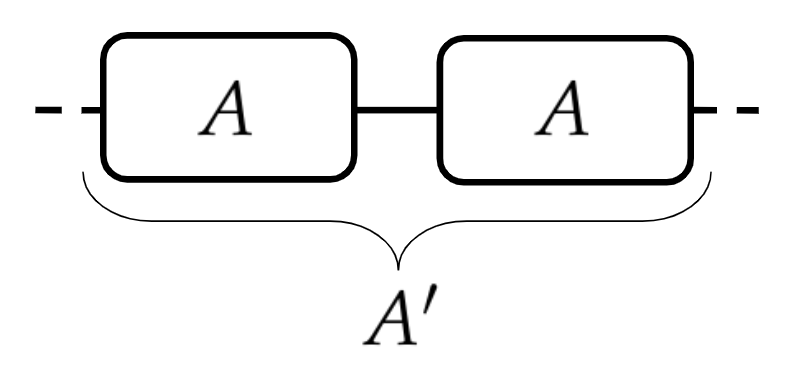
\includegraphics[scale=0.3]{Figures/wilson.png}
    \captionsetup{width=1.\linewidth}
    \caption{Blocking scheme of Wilson's NRG method.}
    \label{fig:wilson}
\end{figure}

First of all, it is important to mention Wilson's numerical renormalization group (NRG) procedure, in which the CSR method is rooted. 

Let us consider a 1D-system made up by $N$ spins. The NRG method suggests to take two spins and consider a subspace of the corresponding Hilbert space $\mathcal{H}_2 \subset \mathcal{H}_1 \otimes \mathcal{H}_1$ of dimension $d_2 \leq d_1^2$; then, one adds a spin and consider the subset of the Hilbert space of three spins $\mathcal{H}_3 \subset \mathcal{H}_2 \otimes \mathcal{H}_1$ of dimension $d_3 \leq d_2d_1$, and so on until one arrives to consider the subset of Hilbert space $\mathcal{H}_N \subset \mathcal{H}_{N-1} \otimes \mathcal{H}_1$ with dimension $d_N \leq d_{N-1}d_1$. So, one can approximate the Hamiltonian with $P_NHP_N$, where the $P_N$ is the projector onto $\mathcal{H}_N$. If one chooses $d_N$ sufficiently small, one can diagonalize the Hamiltonian and find eigenvalues and eigenvectors. A good thing to do is fixing for all the dimensions $d_n$ the so-called \emph{bond dimension} such that 
\begin{equation*}
    d_n \leq D \quad \forall \quad n. 
\end{equation*}

Considering a one-dimensional spin chain,  the NRG method requires to break the chain into a set of identical blocks A (see fig.~\ref{fig:wilson}). So, one diagonalizes the Hamiltonian matrix $H_{AA}$ for two neighboring blocks $A$ and uses its lowest $m$ eigenstates (ordered by energy) to form a pseudo-unitary matrix $O$, employed to change the basis and make up the Hamiltonian $H_{A'}$ representing the block $A'$ twice as large (see fig.~\ref{fig:wilson}), in this way:
\begin{equation*}
    H_{A'} = OH_{AA}O^\dagger,
\end{equation*}
where $O$ is a $m\times n$ matrix (the rows of $O$ are the $m$ lowest eigenstates of $H_{AA}$) and $H_{AA}$ has dimension $n \times n$. This procedure has to be repeated using the new larger blocks $A'$ and the new effective Hamiltonian $H_{A'}$. 

\begin{figure}[H]
\centering
%\begin{subfigure}{6cm}
    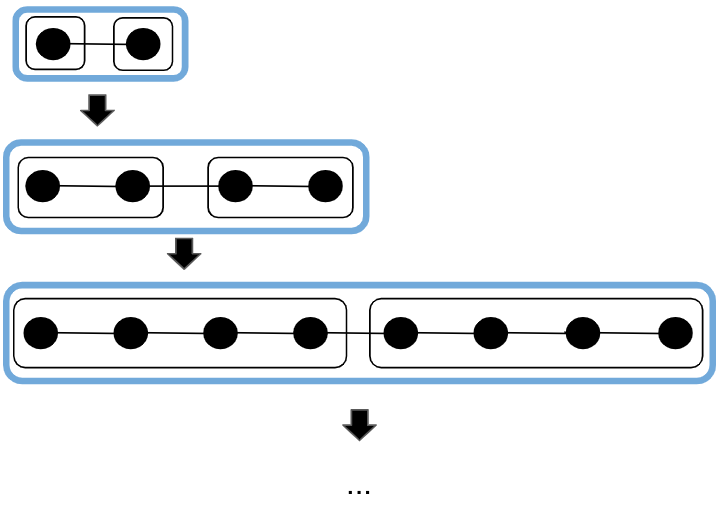
\includegraphics[scale=0.5]{Figures/blocks_wilson}
    \captionsetup{width=1.\linewidth}
    \caption{Merging of the blocks in NRG procedure.}
    \label{fig:blocks_wilson}
%\end{subfigure}\quad
%\begin{subfigure}{6cm}
%    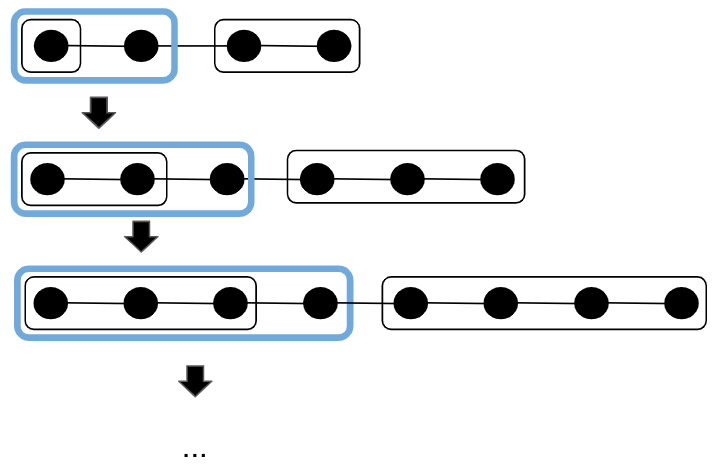
\includegraphics[width=\linewidth]{Figures/blocks_dmrg}
%    \caption{Merging of blocks (block+single site) in DMRG procedure.}
%    \label{fig:blocks_dmrg}
%\end{subfigure}
%\caption{Comparisons of blocking schemes of NRG and DMRG methods.}
%\label{fig:blocks}
\end{figure}

It is worth noting that the NRG method overlooks the connections between the blocks (see fig.~\ref{fig:blocks_wilson}), so it is a good method only in the limit that the links between the blocks vanish. This weak point has been studied and overcome by White in~\cite{s_white:dmrg} where he developed the DMRG method, that will be outlined in the following section.

The CSR method can be seen as a generalization of the NRG method, a development to the case of open systems. The name refers to the idea of selecting a \emph{corner} of the Hilbert space for a lattice system, using eigenvectors of the steady-state density matrix of smaller lattices.

Let us start considering two blocks of a quantum system consisting in a certain number $N$ of sites. The CSR approach is a recursive process that begins with the calculation of the steady-state density matrix of a small block (the first \emph{block} will be a single site, in the second iteration it will be a small lattice constituted of the two blocks emerged in the previous iteration, and so on); this calculation can be done studying the spectrum of the eigenvalue of the Liouvillian and taking the zero value, considered that
\begin{equation}
    \frac{d\rho}{dt} = \mathcal{L} \rho
\end{equation}
can be seen as an eigenvalue equation.

We now consider two spatially adjacent sites: the site A and the site B. We now call $\rho_{A}$ the steady-state density matrix of the first site and $\rho_{B}$ of the latter site. In order to spatially merge these two sites, let us write $\rho_{A}$ and $\rho_{B}$ in terms of an orthonormal basis; if there is no degeneracy among eigevalues of $\rho_{A}$ and $\rho_B$, we can use the orthonormal basis formed by their eigenvectors. Instead, if there is degeneration, a Gram-Schmidt orthonormalization process can be used to obtain an orthonormal basis starting from the ensemble of eigenvectors.

In this way, we will have:
\begin{equation}
    \begin{split}
        \rho_A & = \sum_r p_r^{(A)}\ket{\phi_r^{(A)}}\bra{\phi_r^{(A)}}, \\
        \rho_B & = \sum_{r'} p_{r'}^{(B)}\ket{\phi_{r'}^{(B)}}\bra{\phi_{r'}^{(B)}},
    \end{split}
\end{equation}
where
\begin{equation*}
    \begin{split}
        p_r^{(A)} \geq 0 \quad \forall r \quad &\textrm{and} \quad p_{r'}^{(B)} \geq 0 \quad\forall r', \\
        \sum_{r} p_r^{(A)} = 1 \quad &\textrm{ and } \quad \sum_{r'} p_{r'}^{(B)} = 1.
    \end{split}
\end{equation*}
The steady-state density matrix of the \emph{merged block} constituted of the block A and the block B will be the following:
\begin{equation}
\label{rhoAUB}
    \rho_{AUB} = \rho_A \otimes \rho_B
    = \sum_{r} \sum_{r'} p_r^{(A)}p_{r'}^{(B)}\ket{\phi_r^{(A)}}\ket{\phi_{r'}^{(B)}} \otimes \bra{\phi_{r'}^{(B)}}\bra{\phi_{r}^{(A)}}
\end{equation}

At this point, the CSR method suggests to delineate the \emph{corner-space}; for this purpose, we consider the $M$ most probable product states coming from equation~\ref{rhoAUB} of the form $\ket{\phi_{r}^{(A)}}\ket{\phi_{r'}^{(B)}}$, i.e. we rank them according to the joint probability $p_r^{(A)}p_{r'}^{(B)}$. The $M$ states form an orthonormal basis that generates a subspace
\begin{equation}
\label{basis_corner}
    \Bigl\{\ket{\phi_{r_1}^{(A)}}\ket{\phi_{r_1'}^{(B)}}, \ket{\phi_{r_2}^{(A)}}\ket{\phi_{r_2'}^{(B)}}, \dots, \ket{\phi_{r_M}^{(A)}}\ket{\phi_{r_M'}^{(B)}} \Bigl\},
\end{equation}
called \emph{corner-space}, with
\begin{equation*}
    p_r_1^{(A)}p_{r_1'}^{(B)} \geq p_r_2^{(A)}p_{r_2'}^{(B)} \geq \dots \geq p_r_M^{(A)}p_{r_M'}^{(B)}.
\end{equation*}
So, now it becomes necessary doing a change of basis to the new block $A \cup B$, that is:
\begin{equation}
    H' = \widetilde{O} H_{A\cup B} \widetilde{O}^\dagger,
\end{equation}
where $\widetilde{O}$ is a pseudo-unitary\footnote{The matrix $\widetilde{O}$ is called pseudo-unitary because it is not a square matrix.} $M\times N$ matrix, where $N$ is the dimension of $H_{A\cup B}$; $\widetilde{O}$ is formed by the $M$ eigenvectors of $\rho_{A\cup B}$ living in the corner-space. This density matrix can now be used to calculate the expectation values of any observable.

The larger is $M$, the closer to exactness are the results, because the basis~\ref{basis_corner} spans a larger part of the Hilbert space. Therefore, at this point the value of $M$ should be increased until the convergence is reached.

In the work of~\cite{PhysRevLett.115.080604} it has been proved that convergence can be achieved with a number of states $M$ much smaller than the dimension of the Hilbert space. In the present thesis, it will be shown that this method can not be used for the analysis of systems described by a model such as that under consideration in the present work.

%The resulting dimension of the space in which, from now on - re-iterating the procedure - the system will be studied, is made smaller.

\begin{figure}
    \centering
    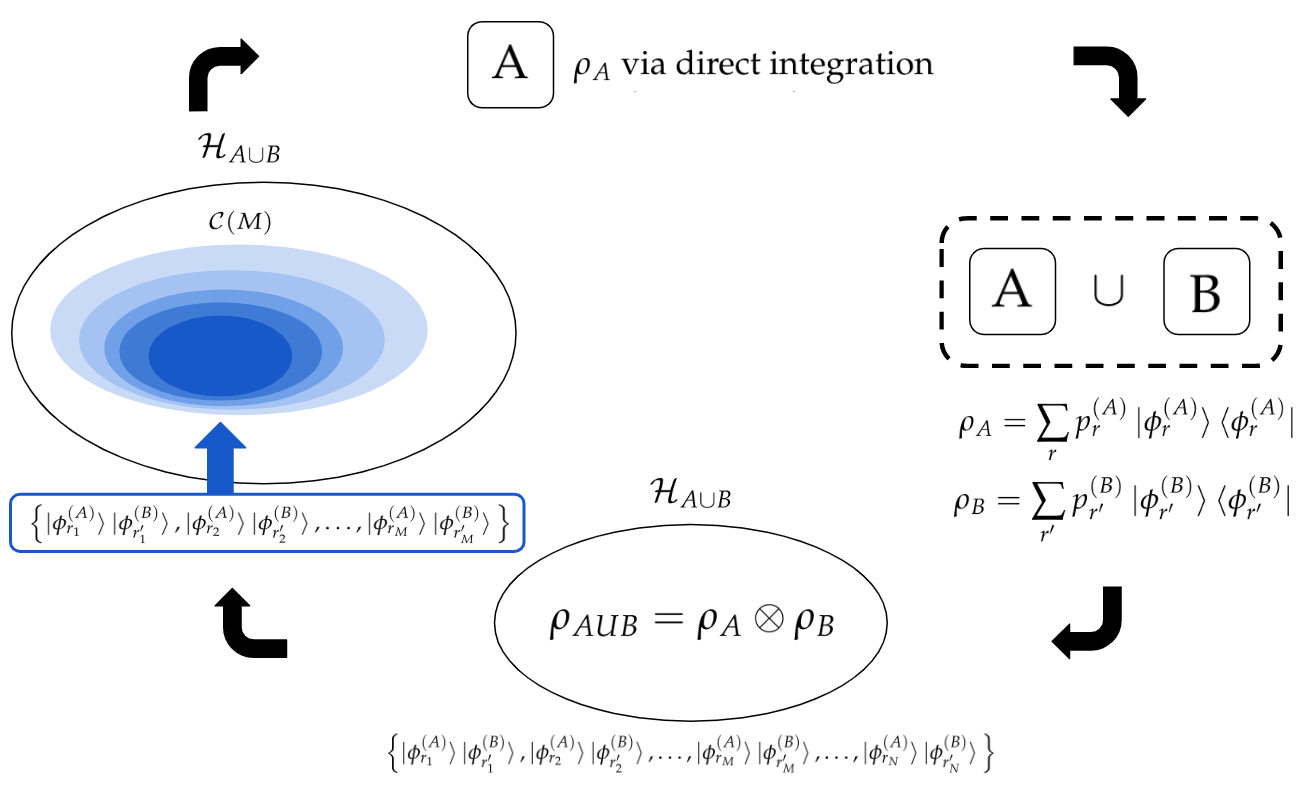
\includegraphics[scale=0.55]{Figures/csr_sketch}
    \captionsetup{width=1.\linewidth}
    \caption{Sketch of the corner-space renormalization method.}
    \label{fig:csr_sketch}
\end{figure}

\bigskip
In short, the algorithm is structured in the following stages, as sketched in fig.~\ref{fig:csr_sketch}:
\begin{description}
    \item[calculation] of the steady-state density matrix of a single block of the system;
    \item[merger] of two predetermined blocks;
    \item[expression] of the density matrix of the merged block in an orthonormal basis;
    \item[selection] of the M most probable states as a basis for the so-called \emph{corner-space};
    \item[increase] of the dimension M of the corner-space until the convergence of the observable is achieved.
\end{description}

A detailed description of the implementation of the algorithm can be seen in Appendix~\ref{AppendixA}.


%%%%%%%%%%%%%%%%%%%%%%%%%%%%%%%%%%%%%%%%%%%%%%%%%%%%%%%%%%%%%%%%%%%%%%%%%%%%%%%%%%%%%%%%%%%%%%%%%%%%%%%%%%%%%%%%%%%%%%%%%%%%%%%%%%%%%%%%%%%%%%%%%%%%%%%%%%%%%%%%%%%%%%%%%%%%%%%%%%%%%%%%%%%%%%%%
\section{The Matrix Product Density Operators (MPO) Method}
\label{chap_numMethods_MPO}
The \emph{matrix product density operator} (MPO) method is rooted in one of the first and most efficient numerical methods to simulate strongly correlated quantum one dimensional systems: the \emph{density matrix renormalization group} (DMRG)~\cite{s_white:dmrg, PhysRevB.48.10345, RevModPhys.77.259}.

Essentially, the DMRG is a generalization of Wilson's NRG method; its core lies in the construction of the so-called \emph{superblock} (see fig.~\ref{fig:DMRG_superblockSketch}): it is constructed in an iterative way, taking a portion of the system, then enlarging it until the desired size is reached; this superblock is usually indicated as $A \bullet \bullet B$. By numerical diagonalization of $H_{A \bullet \bullet B}$ one can find the ground state $\ket{\Psi_{GS}}$ that minimize the energy:
\begin{equation*}
    E = \bra{\Psi_{GS}} H_{A \bullet \bullet B}\ket{\Psi_{GS}}.
\end{equation*}
Since we do not want an exponential increase of the dimension of the Hilbert space, we choose the D most relevant states for block $A \bullet$ (similarly for $\bullet B$). So, having the reduced density operator for $A \bullet$:
\begin{equation*}
    \rho_{A \bullet} = \Tr_{\bullet B} \ket{\Psi_{GS}}\bra{\Psi_{GS}},
\end{equation*}
one uses the D eigenstates with the largest weight (i.e. with the largest eigenvalues) to construct the pseudo-unitary matrix O, useful to truncate the basis:
\begin{equation*}
    H_{A'} = OH_{A\bullet}O^\dagger.
\end{equation*}
At this point, one can replace the first block with the new $A'$.
%\textcolor{red}{REVIEW}

\begin{figure}[H]
    \centering
    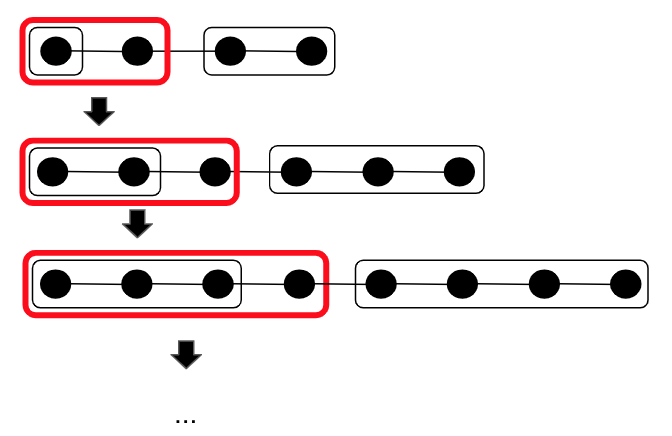
\includegraphics[scale=0.5]{Figures/dmrg_superblock_sketch.png}
    \captionsetup{width=1.\linewidth}
    \caption{Sketch of superblocks formation in DMRG method.} %\textcolor{red}{TO DO: labels to blocks}%The rectangles represent block of $l$ and $l'$ sites respectively, while the circles represent single sites.
    \label{fig:DMRG_superblockSketch}
\end{figure}

%DMRG si può vedere come una riformulazione dei MPS come algoritmo variazionale; l'algoritmo scritto sopra può essere riformulato nell'ottica MPS come algoritmo variazionale
The DMRG method can be expressed as a variational algorithm on a particular class of quantum states, the so-called \emph{matrix product states}~\cite{SCHOLLWOCK201196}.
The MPO method is the generalization of the \emph{matrix product states} (MPS) method \cite{SCHOLLWOCK201196}, which is useful in the description of (closed) quantum many-body systems. The essential idea~\cite{Cirac_2009} behind the MPS techniques lies in Wilson's renormalization group, already mentioned in sec.~\ref{chapter3_csr}.
So, let us consider two spins and a subspace of the corresponding Hilbert space $\mathcal{H}_2 \subset \mathcal{H}_1 \otimes \mathcal{H}_1$ of dimension $d_2 \leq d_1^2$; we write an arbitrary orthonormal basis $\{\ket{\beta}\}_{\beta=1}^{d_2}$ as
\begin{equation*}
    \ket{\beta}_2 = \sum_{n_1, n_2}^{d_{1}} B_\beta^{n_1, n_2} \ket{n_1}_1 \otimes \ket{n_2}_1,
\end{equation*}
where $B_\beta^{n_1, n_2}$ are the coefficients of the basis vectors in terms of the original basis vectors $\ket{n} \in \mathcal{H}_1$ and can be expressed as
\begin{equation*}
    B_\beta^{n_1, n_2} = \sum_{\alpha=1}^{d_{1}} A[1]_\alpha^{n_1}A[2]_{\alpha,\beta}^{n_2},
\end{equation*}
where $A[1]_\alpha^{n_1} = \delta_{n1, \alpha}$ and $A[2]_{\alpha,\beta}^{n_2} = B_\beta^{\alpha, n_2}$. So, we can now write any orthonormal basis in $\mathcal{H}_3$ in terms of $\ket{\beta}_2\otimes \ket{n_3}$ and go on iteratively. After M steps, we have:
\begin{equation*}
    \ket{\beta}_M = \sum_{\alpha=1}^{d_{M-1}}\sum_{n_M=1}^{d_1} A[M]_{\alpha,\beta}^{n_M}\ket{\alpha}_{M-1}\otimes\ket{n_M}_1,
\end{equation*}
that is, substituting recursively the definition of $\ket{\alpha}_m$:
\begin{equation*}
    \ket{\beta}_N = \sum_{n_1,\dots,n_N=1}^{d_1} (A_1^{n_1}A_2^{n_2}\dots A_N^{n_N})_\beta \ket{n_1,\dots,n_N},
\end{equation*}
i.e.
\begin{equation}
\label{mps_general}
    \ket{\psi_{MPS}} = \sum_{n_1,\dots,n_N=1}^{d_1} A_1^{n_1}A_2^{n_2}\dots A_N^{n_N} \ket{n_1,\dots,n_N}.
\end{equation}
Because of this form, such kind of state is called a \emph{matrix product states} (MPS). %\textcolor{red}{FIGURA DAL CIRAC2009 PAGINA 16}

For periodic boundary conditions the form of the~\ref{mps_general} is obtained performing the trace over their product~\cite{SCHOLLWOCK201196, PhysRevLett.93.207204}:
\begin{equation}
    \ket{\psi_{MPS}} = \sum_{n_1,\dots,n_N=1}^{d} \Tr(A_1^{n_1}A_2^{n_2}\dots A_N^{n_N}) \ket{n_1,\dots,n_N}.
\end{equation}
One should note that the total number of parameters turns out to be linear in $N$, i.e. it is equals to $N \times d \times D^2$, $D$ being the bond dimension already mentioned in sec.~\ref{chapter3_csr}; it represents asymptotically the dimension of matrices $A_i^{[k]}$.

Another way of considering the expression~\ref{mps_general} is the graphical notation to represent the operators $A^{[k]}_i$ sketched in figure~\ref{fig:mps_graphical}. Here, every operator is represented by a square with 3 legs: there are two of them for the bonds with the neighbouring operators, the other one for the physical index. 

\begin{figure}[H]
    \centering
    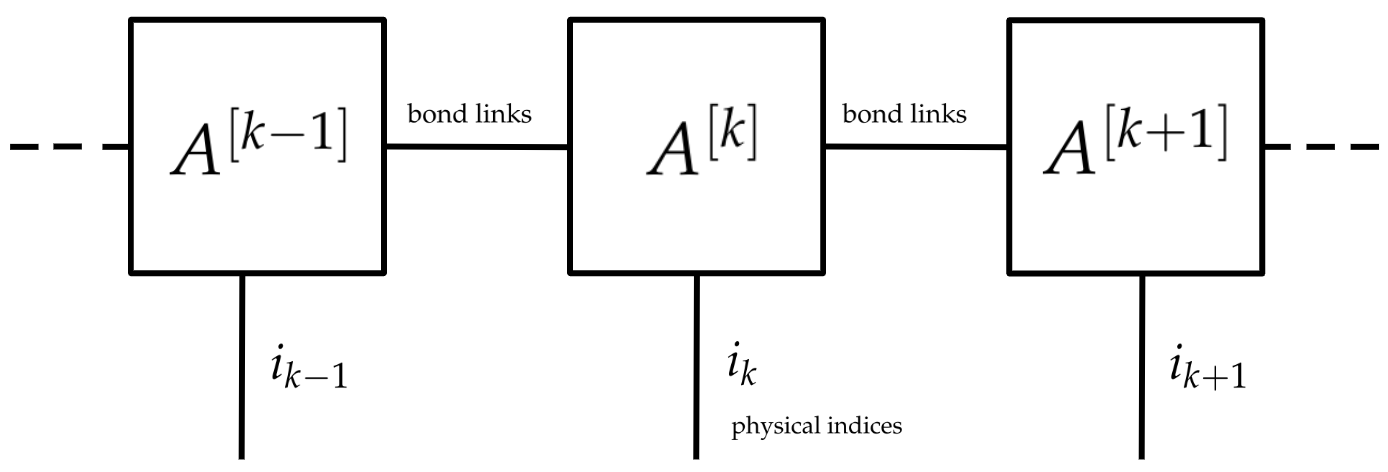
\includegraphics[scale=0.4]{Figures/mps_graphical.png}
    \captionsetup{width=1.\linewidth}
    \caption{Graphical representation of an MPS in terms of tensor network.}
    \label{fig:mps_graphical}
\end{figure}

The matrix product \emph{density operators} (MPO) extend the MPS from pure to mixed states, following the idea explained, for example, in~\cite{PhysRevLett.93.207204, MPO_method}. The physical index is now doubled, as illustrated in fig.~\ref{fig:mpo_graphical}
\begin{equation}
\label{eqn:mpdo}
    \rho_{MPO} = \sum_{i_1, \dots ,i_N = 1}^{d} \sum_{j_1, \dots ,j_N = 1}^{d} \Tr\Bigl(A_1^{i_1,j_1} \dots A_N^{i_N,j_N}\Bigl) \ket{i_1, \dots ,i_N}\bra{j_1, \dots ,j_N}.
\end{equation}
The $A^{[k]i_k,j_k}$ are $D^2 \times D^2$ tensors that can be decomposed in this way:
\begin{equation*}
    A_k^{i,j} = \sum_{a = 1}^{d_k} M_k^{i,a} \otimes (M_k^{j,a})^*.
\end{equation*}

Also in this case, there is a graphical notation to represent the tensors $A^{[k]}_{i,j}$ ske-tched in figure~\ref{fig:mpo_graphical}. Here, every tensor is represented by a square with 4 legs: there are two of them for the bonds with the neighbouring tensors, the other two for the physical indices (the "bras" and "kets"). 

\begin{figure}[H]
    \centering
    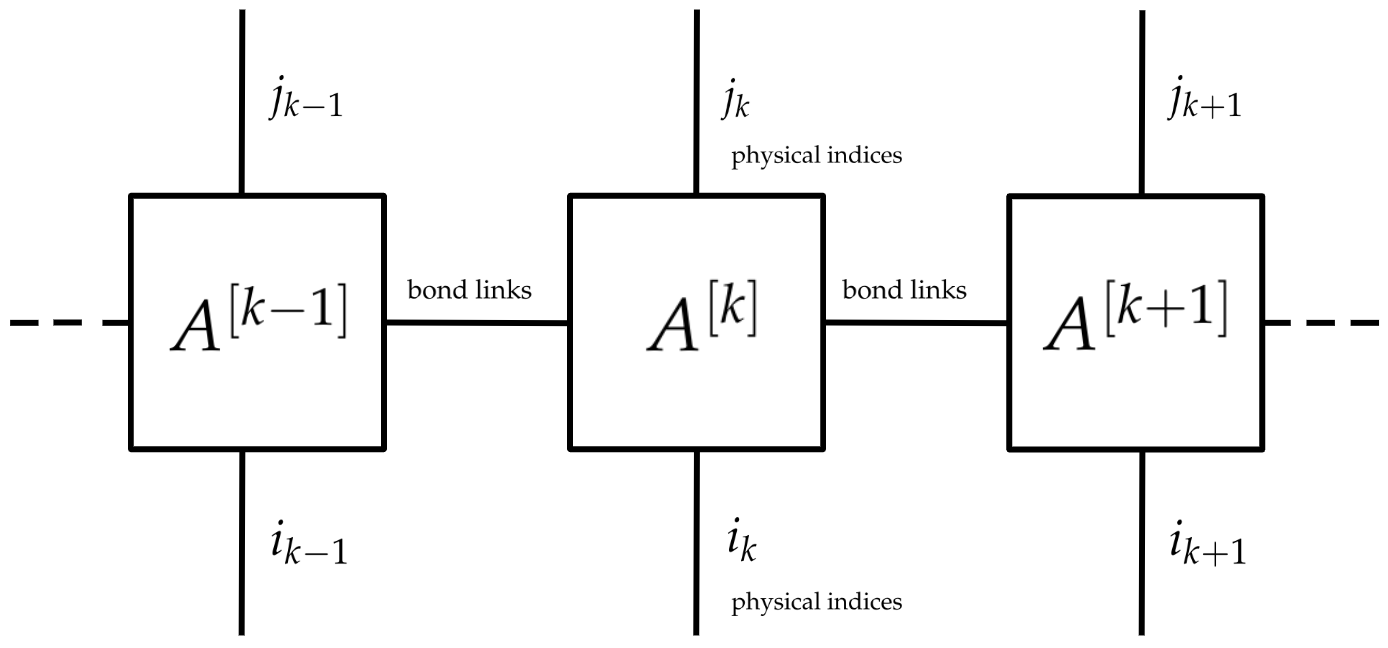
\includegraphics[scale=0.4]{Figures/mpo_graphical.png}
    \captionsetup{width=1.\linewidth}
    \caption{Graphical representation of an MPO in terms of tensor network.}
    \label{fig:mpo_graphical}
\end{figure}

As regards the dynamics, the long-time limit of eq.~\ref{eqn:lindblad_eqn} can be reached using a MPO ansatz for the density matrix. The steady-state solution $\rho$ is found using an algorithm based on the \emph{time evolution block decimation} (TEBD)~\cite{PhysRevLett.91.147902} scheme adapted to open systems. It is useful to efficiently compute time-dependent properties of 1D closed quantum many-body systems as done in~\cite{PhysRevLett.93.040502}. 

Here, we can briefly see how it works~\cite{jin_biella_ross} in the case of open many-body systems in the MPO formalism. 

First of all, let us consider the expression~\ref{eqn:mpdo}: repeated single-value decomposition of the tensor $A^{i_1,\dots, i_N; j_1,\dots, j_N}$ can lead to
\begin{equation*}
\label{mpo_ansatz}
\begin{split}
    \rho_{MPO} = \sum_{i_1, \dots ,i_N = 1}^{d}\quad \sum_{j_1, \dots ,j_N = 1}^{d}\quad &\sum_{\alpha_1,\dots, \alpha_{N-1} = 1}^\chi (\Gamma_{1, \alpha_1}^{[1]i_1, j_1}\lambda_{\alpha_1}^{[1]})(\Gamma_{\alpha_1, \alpha_2}^{[2]i_, j_2}\lambda_{\alpha_2}^{[2]}) \dots \\  \times &(\lambda_{\alpha_{N-1}}^{[N-1]}\Gamma_{N, \alpha_{N-1}}^{[N]i_N, j_N}) ||i_1, \dots ,i_N, j_1, \dots ,j_N\rangle\rangle,
    \end{split}
\end{equation*}
where the superoperator formalism\footnote{Every linear operator $A$ acting on the Hilbert space $\mathcal{H}$ can be associated with a vector in a superoperator space~\cite{davRoss_wordpress}:
\begin{equation*}
    A = \sum_{ij} A_{ij} \ket{i}\bra{j} \quad \rightarrow \quad |A\rangle\rangle = \sum_{ij} A_{ij} \ket{i}\ket{j}.
\end{equation*}} has been used in order to write the superket \\$||i_1, \dots ,i_N, j_1, \dots ,j_N\rangle\rangle$. The bond-link dimension $\chi$ can be kept under a threshold by discarding the smallest single values; moreover, it is proportional to the amount of quantum correlations between the system sites that can be embedded in $\rho_{MPO}$. As said in sec.~\ref{bi_mixed_states}, the operator space entanglement entropy is a good quantifier of this aspect; in particular, the smaller is its value, the better is the functionality of the MPO method.

%As shown in~\cite{Prosen_2009, PhysRevLett.93.207205}, $\hat{\mathcal{L}}$ %can be decomposed into terms that involve two contiguous sites, as
%\begin{equation}
%    \hat{\mathcal{L}}[\rho] = \sum_l \hat{\mathcal{L}}_{l,l+1}[\rho].
%\end{equation}
Formally, the solution of~\ref{eqn:lindblad_eqn} can be written as
\begin{equation}
\label{eqn:lindblad_dinamics}
    \rho(t) = e^{\mathcal{L}t}\rho(0).
\end{equation}
Following the Vidal's work~\cite{PhysRevLett.93.040502}, the liouvillian superoperator $\mathcal{L}$ can be decomposed in this way:
\begin{equation}
    \mathcal{L} = F + G,
\end{equation}
where
\begin{equation}
    \begin{split}
        F &\equiv \sum_{\text{even } l} (\mathcal{L}^{l, l+1}) \\
        G &\equiv \sum_{\text{odd } l} (\mathcal{L}^{l, l+1}), \\
        l  &= 1, \dots N-1
    \end{split}
\end{equation}
having considered a Liouvillian made of arbitrary nearest-neighbouring interaction terms.

For every small time step $\tau > 0$, the Trotter-Suzuki expansion of order $p$ for $\exp{(\mathcal{L} t)}$ reads:
\begin{equation}
    e^{\mathcal{L}t} = e^{(F+ G)t} = e^{[(F+ G)\tau]\frac{t}{\tau}} \approx [f_p(U_{F\tau}, U_{G\tau})]^{\frac{t}{\tau}},
    %\prod_k \exp{(\alpha_k\hat{\mathcal{L}}_1\tau)}\dots\exp{(\beta_k\hat{\mathcal{L}}_N\tau)} + \mathcal{O}(\tau^p),
\end{equation}
%with $p$ depending on the required accuracy.
where $U_{F\tau} \equiv e^{F\tau}$ and $U_{G\tau} \equiv e^{G\tau}$ and where
\begin{equation}
    f_1(x,y) = xy, \quad f_2(x, y) = x^{1/2}yx^{1/2}
\end{equation}
for the first and the second order expansions.
The simulation of time evolution~\ref{eqn:lindblad_dinamics} can then be accomplished by iteratively applying $U_{F\tau}$ and $U_{G\tau}$ to $\rho(0)$ a number $\mathcal{O}(\frac{t}{\tau})$ of times.

%\textcolor{red}{VEDI PRESENTAZIONE GARNET CHAN - RIVEDERE \\ AGGIUNGERE FORMALISMO SUPEROPERATORIALE}

%\noindent\rule[0.5ex]{\linewidth}{1pt}
%\noindent\rule[0.5ex]{\linewidth}{1pt}

%One can express a MPDO in terms of a pure state MPS using the \emph{purification}~\cite{nielsen_chuang} technique. The essential idea is to consider an auxiliary system with a Hilbert space of dimension $d_k$ and, after choosing an orthonormal basis $\ket{i_k, a_k}$, to write the corresponding MPS state as
%\begin{equation}
%    \ket{\psi} = \sum_{i_1,\dots,i_N} \sum_{a_1, \dots, a_N} Tr\Bigl(\prod_{k=1}^N B_k^{i_k, a_k}\Bigl) \ket{i_1a_1, \dots, i_Na_N}.
%\end{equation}
%and eventually the MPDO $\rho$ is obtained tracing over the indices referred to the auxiliary system $a_k$:
%\begin{equation}
%    \rho = Tr_a(\ket{\psi}\bra{\psi});
%\end{equation}
%this density matrix can be used to compute the expectation values of observables.